% EXST 7152 - Midterm Project   
% Yuan, Jumao 

\documentclass[11pt]{article}
\usepackage[margin=2.0cm]{geometry}
\usepackage{color,soul}
\usepackage{xcolor}
\usepackage{sectsty}
\usepackage{hyperref}
\usepackage [english]{babel}
\usepackage [autostyle, english = american]{csquotes}
\usepackage{fancyhdr}
\usepackage{setspace}
\usepackage{cite}
\usepackage{url}
\usepackage{float}
\usepackage{amsmath}
\usepackage{csquotes}
\usepackage{geometry}
\usepackage{colortbl}
\usepackage{graphicx} %add png pictures
\usepackage{indentfirst}
\usepackage{graphicx}
\usepackage{eso-pic}% http://ctan.org/pkg/eso-pic
\usepackage{lipsum} % http://ctan.org/pkg/lipsum
\MakeOuterQuote{"}
\sectionfont{\color{red}}
\subsectionfont{\color{blue}}
%\subsubsectionfont{\color{purple}}
\title{Stay Alert! The Ford Challenge\\
       \hfill --\small{Kaggle 2011}}
\author{Yuan, Jumao}
\date{03/31/2015}
\usepackage{Sweave}


\begin{document}
%\begin{singlespacing}
\Sconcordance{concordance:Draft.tex:Draft.Rnw:%
1 54 1 1 3 28 1 1 3 51 1 1 2 6 0 2 1 9 0 1 1 5 0 1 1 1 3 2 0 1 2 1 0 3 %
1 3 0 1 2 6 1 1 3 2 1 1 3 2 1 1 3 2 1 1 3 2 1 1 3 2 1 1 3 3 1 1 3 19 1}

\maketitle

\fancypagestyle{plain}{%
   \fancyhead[R]{\textit{EXST 7152 - Midterm Project}}
   \renewcommand{\headrulewidth}{0pt}
}

\setlength\parindent{0pt} %noindent
\singlespacing

%  Midterm Project will be presented on March, 31th, 2015 (Tuesday)

% setwd('/Users/jumaoyuan/Dropbox/Ford_Alert')
% getwd()

\tableofcontents
\newpage
\doublespacing  %setspace
%------------------------------------ (Abstract) --------------------------------%
\section{Abstract}
The "Stay Alert!" competition from Ford challenged competitors to predict whether a car driver was not alert based on various measured features.\\
The features were presented in 3 sets: physiological(P1~P8), environmental(E1~E11) and vehicular(V1~V11). Each feature was presented as a real number. For each measurement we were also told whether the driver was alert or not at that time(a boolean label called IsAlert).\\
We splitted data into 70\% training data and 30\% testing data. "Area under the curve"(AUC) was used as the accuracy assessment criteria. \\
We used "logistic regression(glmnet in R)", "naive bayes", "classification tree(tree in R)", "random forest"and "SVM" models, and found "random forest" model works much better than others by comparison of AUC scores and ROC curves.

%------------------------------------ (Problem Description) --------------------------------%
\section{Introduction} %background
Driving while distracted, fatigued or drowsy may lead to accidents. Activities that divert the driver's attention from the road ahead, such as engaging in a conversation with other passengers in the car, making or receiving phone calls, sending or receiving text messages, eating while driving or events outside the car may cause driver distraction. Fatigue and drowsiness can result from driving long hours or from lack of sleep.

The objective of this challenge is to design a detector/classifier that will detect whether the driver is alert or not alert, employing any combination of vehicular, environmental and driver physiological data that are acquired while driving.

%------------------------------------ (Import Data) ------------------------------------%
\section{Data Description} %import data
We can download data from website \url{https://www.kaggle.com/c/stayalert/data}. The data for this challenge shows the results of a number of "trials", each one representing about 2 minutes of sequential data that are recorded every 100 ms during a driving session on the road or in a driving simulator.  The trials are samples from some 100 drivers of both genders, and of different ages and ethnic backgrounds. The files are structured as follows:

The first column is the Trial ID - each period of around 2 minutes of sequential data has a unique trial ID. For instance, the first 1210 observations represent sequential observations every 100ms, and therefore all have the same trial ID \\
The second column is the observation number - this is a sequentially increasing number within one trial ID \\
The third column has a value X for each row where   
\begin{itemize}
\item X = 1     if the driver is alert 
\item X = 0     if the driver is not alert 
\end{itemize}
The next 8 columns with headers P1, P2 ,......, P8  represent physiological data;\\
The next 11 columns with headers E1, E2,......, E11  represent environmental data;\\
The next 11 columns with headers V1, V2,......, V11  represent vehicular  data;

%------------------------------------ (Evaluation-AUC) ------------------------------------%
\section{Evaluation}
Entries will be evaluated using the area under the \textbf{receiver operator curve} (AUC). AUC was first used by the American army after the attack on Pearl Harbour, to detect Japanese aircraft from radar signals.

Today, it is a commonly used evaluation method for binary choose problems, which involve classifying an instance as either positive or negative. Its main advantages over other evaluation methods, such as the simpler misclassification error, are:  

1. It's insensitive to unbalanced datasets (datasets that have more installeds than not-installeds or vice versa).

2. For other evaluation methods, a user has to choose a cut-off point above which the target variable is part of the positive class (e.g. a logistic regression model returns any real number between 0 and 1 - the modeler might decide that predictions greater than 0.5 mean a positive class prediction while a prediction of less than 0.5 mean a negative class prediction). AUC evaluates entries at all cut-off points, giving better insight into how well the classifier is able to separate the two classes. \\

\textbf{Understanding AUC}

To understand the calculation of AUC, a few basic concepts must be introduced. For a binary choice prediction, there are four possible outcomes:
\begin{itemize}
\item true positive - a positive instance that is correctly classified as positive;
\item false positive - a negative instance that is incorrectly classified as positive;
\item true negative - a negative instance that is correctly classified as negative;
\item false negative - a positive instance that is incorrectly classified as negative);
\end{itemize}

These possibilities can be neatly displayed in a confusion matrix:

\begin{center}
\begin{tabular}{|l|l|l|}
\hline
  & P             & N \\ \hline
P & true positive & false positive \\ \hline
N & false positive & true positive \\
\hline
\end{tabular}
\end{center}

The true positive rate, or recall, is calculated as the number of true positives divided by the total number of positives. When identifying aircraft from radar signals, it is proportion that are correctly identified.

The false positive rate is calculated as the number of false positives divided by the total number of negatives. When identifying aircraft from radar signals, it is the rate of false alarms.


%------------------------------------ (Preprocessing) ------------------------------------%
\section{Data Preprocessing}
%------------------------------------%
\subsection{Missing values and typos}
Usually, we use data imputation to make up missing values; while, in this problem, not many missing values adn typos exist, so we can just remove them. 

%------------------------------------%
\subsection{Remove redundant variables}
In the original dataset, we can see variables "P8", "V7" and "V9" are redundant. Therefore, we can delete these 3 columns in the data preprocessing.

%------------------------------------%
\subsection{Split into training and testing datasets}
We randomly split data into 70\% test datasets and 30\% training datasets and repeate all models with a few iterations.

\begin{Schunk}
\begin{Sinput}
> getwd()
\end{Sinput}
\begin{Soutput}
[1] "/Users/jumaoyuan/Desktop/All_Proj_7152/Ford_Alert"
\end{Soutput}
\begin{Sinput}
> data <- read.csv(file = "fordTrain.csv")
> names(data)
\end{Sinput}
\begin{Soutput}
 [1] "TrialID" "ObsNum"  "IsAlert" "P1"      "P2"      "P3"      "P4"     
 [8] "P5"      "P6"      "P7"      "P8"      "E1"      "E2"      "E3"     
[15] "E4"      "E5"      "E6"      "E7"      "E8"      "E9"      "E10"    
[22] "E11"     "V1"      "V2"      "V3"      "V4"      "V5"      "V6"     
[29] "V7"      "V8"      "V9"      "V10"     "V11"    
\end{Soutput}
\begin{Sinput}
> dim(data)
\end{Sinput}
\begin{Soutput}
[1] 604329     33
\end{Soutput}
\begin{Sinput}
> newdata <- data[,3:ncol(data)]
> # dim(newdata)
> # names(newdata)
> smp_size <- floor(0.70 * nrow(newdata))
> ## set the seed to make your partition reproductible
> set.seed(123)
> train_ind <- sample(seq_len(nrow(newdata)), size = smp_size)
> training <- newdata[train_ind, ]
> testing <- newdata[-train_ind, ]
\end{Sinput}
\end{Schunk}

%------------------------------------ (Models) ------------------------------------%
\section{Build Moldes}
R code can be accessible on my github repository \url{https://github.com/jyuan4/Amazon_Challenge_Kaggle}.

%---------------- (Logistic Reg) --------------------%
\subsection{Logistic Regression}
\begin{Schunk}
\begin{Sinput}
library(glmnet)
training <- as.matrix(na.omit(training))
testing <- as.matrix(na.omit(testing))
fit <- glmnet(training[,2:ncol(training)], training[,1], family="binomial")
plot(fit)
cv3 <- cv.glmnet(training[,2:ncol(training)], training[,1], family="binomial", type="class")
plot(cv3)
cv3$lambda.min
cv3$lambda.1se
pred2 <- as.vector(predict(fit, testing[,2:ncol(testing)], type="class", s=cv3$lambda.min))
pred2 <- data.frame(pred2)
testing <- data.frame(testing)
glmnet.table <- table(pred2[,1], testing$IsAlert)
1-sum(diag(glmnet.table))/sum(glmnet.table)

library(pROC)
roc.curve <- roc(as.numeric(pred2[,1])-1, testing$IsAlert)
plot(roc.curve, main = "ROC: Logistic Regression", col = "red")
auc.score<-auc(testing$IsAlert, as.numeric(pred2[,1])-1)
auc.score
\end{Sinput}
\begin{Soutput}
[1] 0.7803548
\end{Soutput}
\end{Schunk}

% add ROC curve
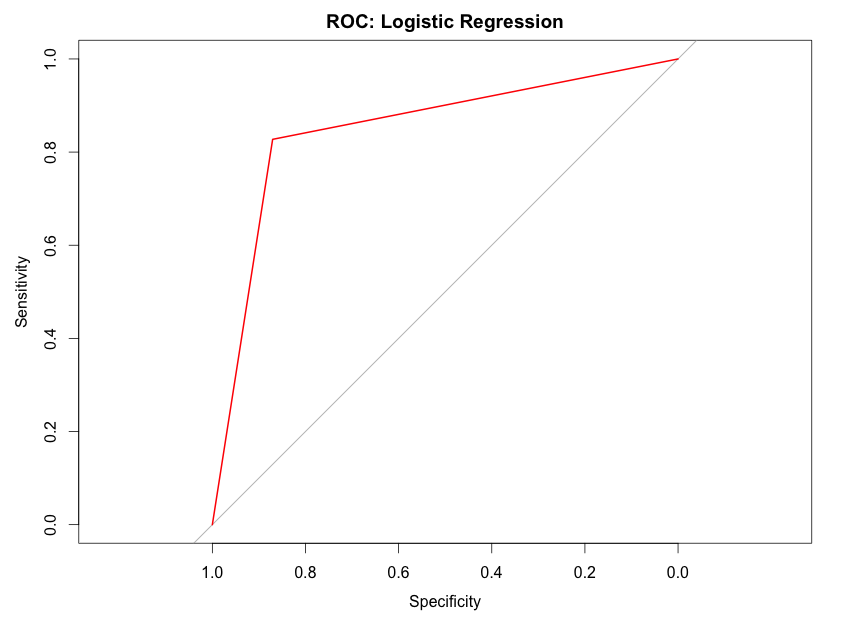
\includegraphics[scale=0.4]{LogReg_ROC.png} \\
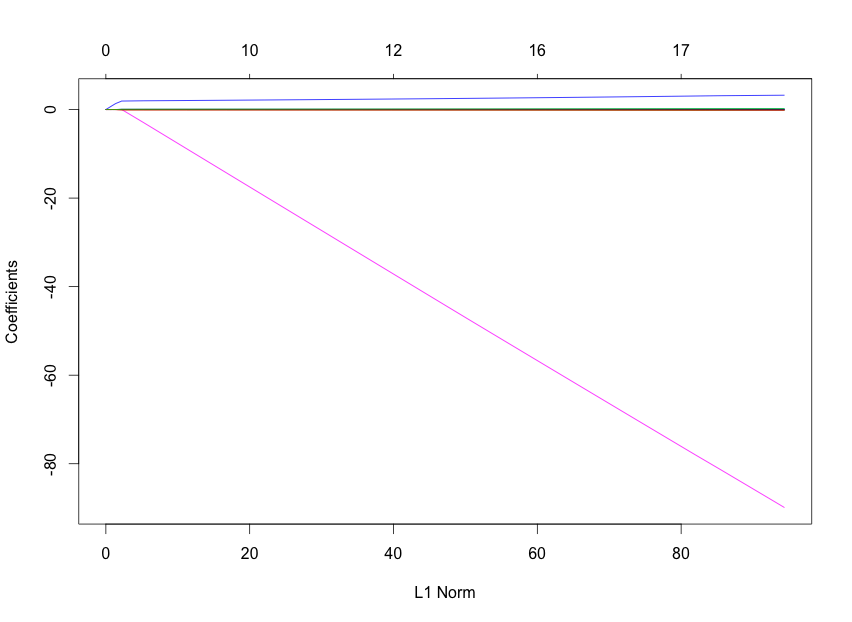
\includegraphics[width=.5\linewidth]{logReg_1.png}
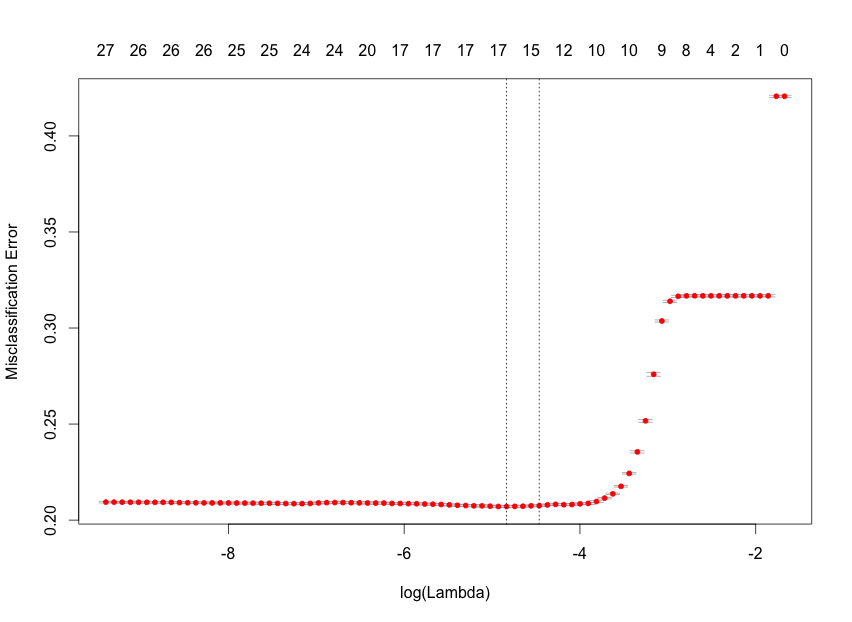
\includegraphics[width=.5\linewidth]{LogReg_2.png}

%---------------- (Classification Tree)--------------------%
\subsection{Classification Tree}
\begin{Schunk}
\begin{Sinput}
library(tree)
training$IsAlert <- factor(training$IsAlert)
tree.fit <- tree(IsAlert~.,data=training)
summary(tree.fit)
plot(tree.fit)
text(tree.fit, pretty=0)
tree.fit
\end{Sinput}
\begin{Soutput}
node), split, n, deviance, yval, (yprob)
      * denotes terminal node

  1) root 423030 575700.0 1 ( 0.42064 0.57936 )  
    2) E9 < 0.5 52071  28520.0 0 ( 0.92199 0.07801 )  
      4) E10 < 59.5 11469  13770.0 0 ( 0.71227 0.28773 ) *
      5) E10 > 59.5 40602   7568.0 0 ( 0.98123 0.01877 ) *
    3) E9 > 0.5 370959 480500.0 1 ( 0.35027 0.64973 )  
      6) V11 < 8.1583 105882 136200.0 0 ( 0.65689 0.34311 )  
       12) V1 < 66.535 22583  22560.0 1 ( 0.19935 0.80065 ) *
       13) V1 > 66.535 83299  87580.0 0 ( 0.78093 0.21907 )  
         26) E10 < 54.5 42735  21530.0 0 ( 0.93069 0.06931 ) *
         27) E10 > 54.5 40564  53750.0 0 ( 0.62316 0.37684 )  
           54) P5 < 0.243249 34241  41550.0 0 ( 0.70489 0.29511 ) *
           55) P5 > 0.243249 6323   5973.0 1 ( 0.18061 0.81939 ) *
      7) V11 > 8.1583 265077 284500.0 1 ( 0.22779 0.77221 )  
       14) V11 < 12.5697 121332 157300.0 1 ( 0.35145 0.64855 )  
         28) V11 < 10.6767 76957  83710.0 1 ( 0.23383 0.76617 ) *
         29) V11 > 10.6767 44375  60970.0 0 ( 0.55543 0.44457 )  
           58) P6 < 718 20841  23710.0 1 ( 0.25594 0.74406 ) *
           59) P6 > 718 23534  22140.0 0 ( 0.82064 0.17936 )  
            118) P5 < 0.205626 21771  15540.0 0 ( 0.88498 0.11502 ) *
            119) P5 > 0.205626 1763    426.2 1 ( 0.02609 0.97391 ) *
       15) V11 > 12.5697 143745 107400.0 1 ( 0.12341 0.87659 ) *
\end{Soutput}
\begin{Sinput}
set.seed(2)
testing$IsAlert <- as.factor(testing$IsAlert)
tree.pred <- predict(tree.fit, testing, type="class")
tree.table <- table(tree.pred, testing$IsAlert)

library(pROC)
roc.curve <- roc(as.numeric(tree.pred)-1, as.numeric(testing$IsAlert)-1)
plot(roc.curve, main = "ROC: Classification Tree", col = "red")
auc.score<-auc(as.numeric(testing$IsAlert)-1, as.numeric(tree.pred)-1)
auc.score
\end{Sinput}
\begin{Soutput}
[1] 0.8287284
\end{Soutput}
\end{Schunk}

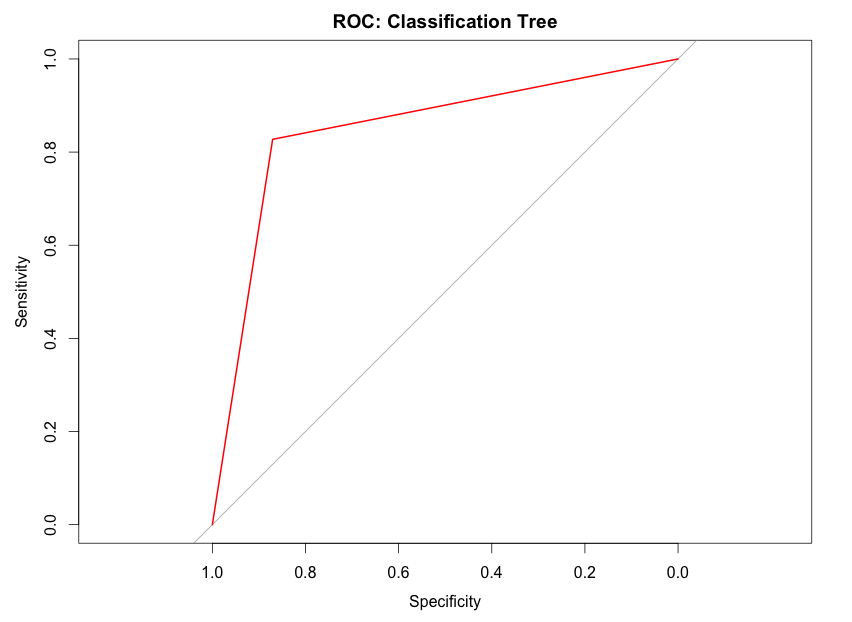
\includegraphics[scale=0.5]{ClassTree_ROC.png} \\
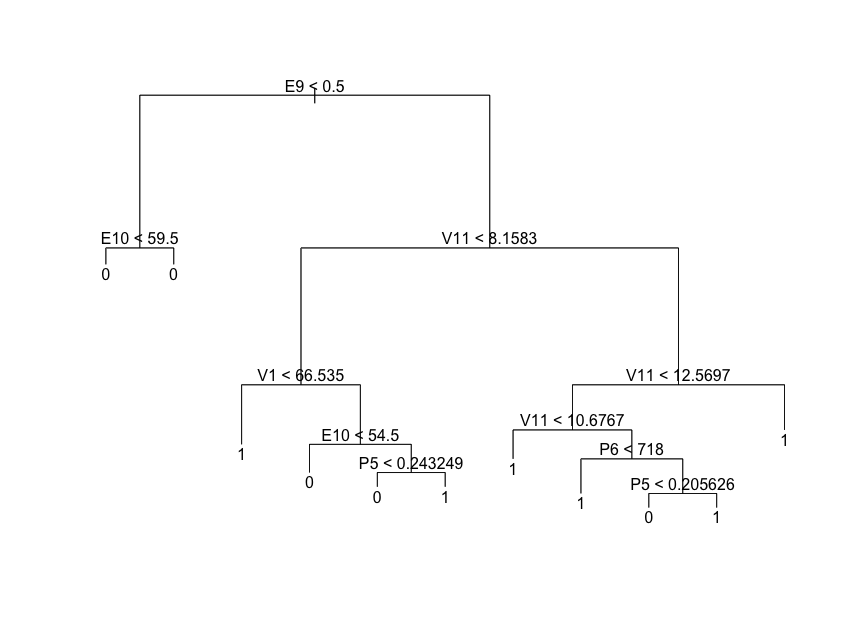
\includegraphics[scale=0.5]{ClassTree_Plot.png}

%---------------- (GLM)--------------------%
\subsection{GLM}
\begin{Schunk}
\begin{Sinput}
training <- data.frame(training)
training <- na.omit(training)
lr.fit <- glm(IsAlert~., data=training)
summary(lr.fit)
#P8, V7 and V9 are redundant/useless variables

testing <- data.frame(testing)
testing <- na.omit(testing)
lr.pred <- predict(lr.fit, testing[,-1], type="response")

lr.pred[lr.pred>=0.5] <- 1
lr.pred[lr.pred<0.5] <- 0
lr.table <- table(lr.pred, testing$IsAlert)
1-sum(diag(lr.table))/sum(lr.table) #misclassification rate

library(pROC)
set.seed(100)
roc.curve <- roc(as.numeric(lr.pred), testing$IsAlert)
plot(roc.curve, main = "ROC: GLM", col = "red")
auc.score<-auc(as.numeric(testing$IsAlert), as.numeric(lr.pred))
auc.score
\end{Sinput}
\begin{Soutput}
[1] 0.741541
\end{Soutput}
\end{Schunk}

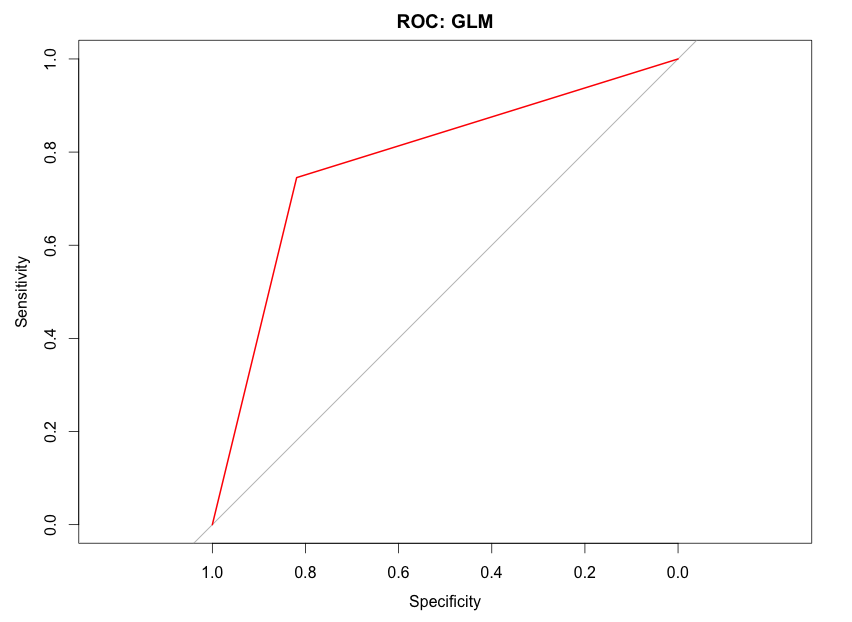
\includegraphics[scale=0.5]{GLM_ROC.png} 

%---------------- (RF)--------------------%
\subsection{Random Forest}
\begin{Schunk}
\begin{Sinput}
library(randomForest)
set.seed(100)
#100 ntree - slow iterations
RF <- randomForest(training[,-c(1,9,27,29)], factor(training$IsAlert),
                   sampsize=10000, do.trace=TRUE, importance=TRUE, ntree=100, forest=TRUE)         
varImpPlot(RF)
rf.pred <- data.frame(IsAlert.pred=predict(RF,testing[,-c(1,9,27,29)],type="prob")[,2])

library(pROC)
set.seed(10)
roc.curve <- roc(rf.pred[,1], as.numeric(testing$IsAlert))
plot(roc.curve, main = "ROC: RF", col = "red")
auc.score<-auc(as.numeric(testing$IsAlert), rf.pred[,1])
auc.score

rf.pred[rf.pred>=0.5] <- 1
rf.pred[rf.pred<0.5] <- 0
rf.table <- table(pred=rf.pred[,1], testing$IsAlert)
1-sum(diag(rf.table))/sum(rf.table) #misclassification rate
\end{Sinput}
\begin{Soutput}
[1] 0.9293929
\end{Soutput}
\end{Schunk}

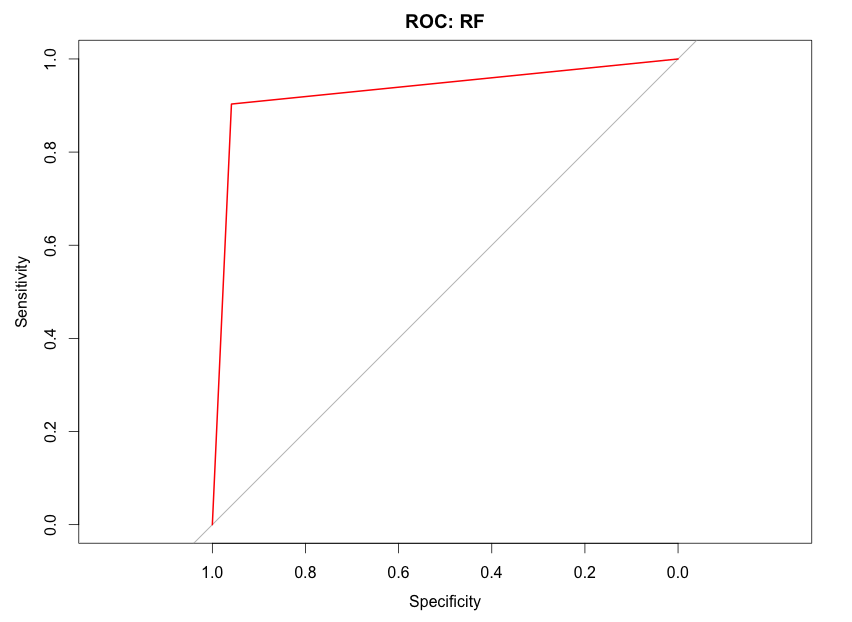
\includegraphics[scale=0.5]{RF_ROC.png}\\
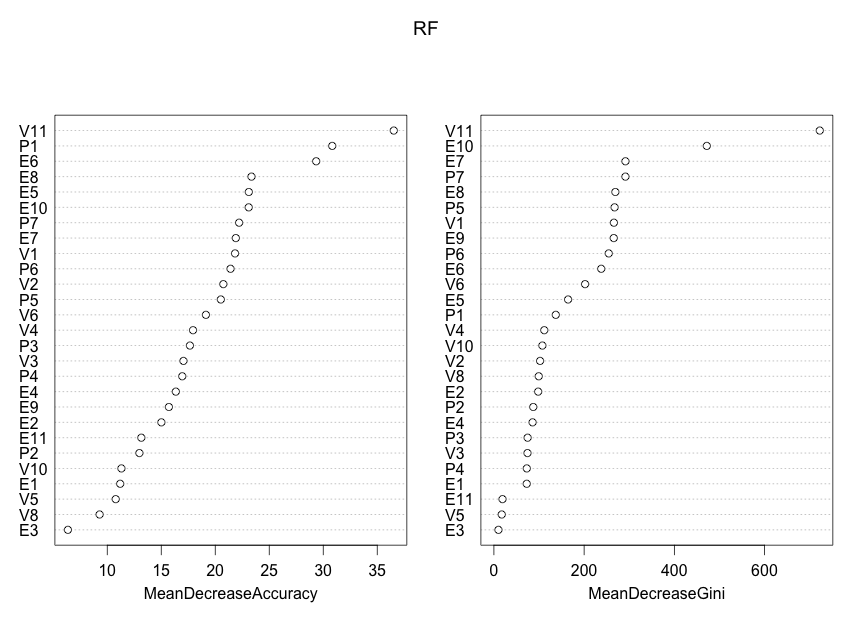
\includegraphics[scale=0.5]{RF_importance.png}

%---------------- (Naive Bayes)--------------------%
\subsection{Naive Bayes}
\begin{Schunk}
\begin{Sinput}
#http://stackoverflow.com/questions/20091614/naive-bayes-classifier-in-r
## Categorical data only
library(e1071)
# training$IsAlert[training$IsAlert==1] <- 'TRUE'
# training$IsAlert[training$IsAlert==0] <- 'FALSE'
# testing$IsAlert[testing$IsAlert==1] <-  'TRUE'
# testing$IsAlert[testing$IsAlert==0] <- 'FALSE'
training <- na.omit(training)
testing <- na.omit(testing)
training <- data.frame(training)
testing <- data.frame(testing)
training$IsAlert <- as.factor(training$IsAlert)
testing$IsAlert <- as.factor(testing$IsAlert)
model <- naiveBayes(IsAlert~., data=training)
NB.pred <- predict(model, testing)
NB.table <- table(NB.pred, testing$IsAlert)
1-sum(diag(NB.table))/sum(NB.table)

library(pROC)
roc.curve <- roc(as.numeric(NB.pred)-1, as.numeric(testing$IsAlert)-1)
plot(roc.curve, main = "ROC: Naive Bayes", col = "red")
auc.score<-auc(as.numeric(testing$IsAlert)-1, as.numeric(NB.pred)-1)
auc.score
\end{Sinput}
\begin{Soutput}
[1] 0.6774233
\end{Soutput}
\end{Schunk}

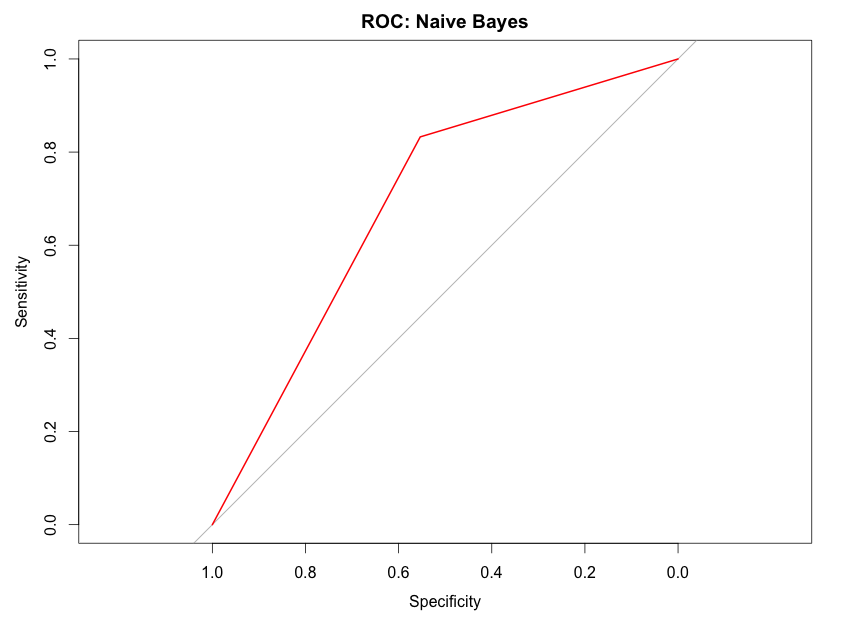
\includegraphics[scale=0.5]{ROC_NaiveBayes.png} 

%---------------- (CART - regression tree)--------------------%
\subsection{CART}
\begin{Schunk}
\begin{Sinput}
library(rpart) #grow a regression tree
set.seed(1)
training <- data.frame(training)
rpart.fit <- rpart(IsAlert~., data=training, control=rpart.control(minsplit = 10))
par(xpd=NA)
plot(rpart.fit, uniform = T)
text(rpart.fit, use.n = TRUE)

set.seed(2)
testing$IsAlert <- as.factor(testing$IsAlert)
rpart.pred <- predict(rpart.fit, testing, type="class")
rpart.table <- table(rpart.pred, testing$IsAlert)
1-sum(diag(rpart.table))/sum(rpart.table)

library(pROC)
roc.curve <- roc(as.integer(rpart.pred)-1, as.numeric(testing$IsAlert)-1)
plot(roc.curve, main = "Logistic Regression ROC Curve", col = "red")
auc.score<-auc(as.numeric(testing$IsAlert)-1, as.numeric(rpart.pred)-1)
auc.score

library("partykit")
plot(as.party(rpart.fit), tp_args = list(id=FALSE))
print(rpart.fit$cptable)
opt <- which.min(rpart.fit$cptable[,"xerror"])
cp <- rpart.fit$cptable[opt, "CP"]
rpart_prune <- prune(rpart.fit, cp=cp)
plot(as.party(rpart_prune), tp_args = list(id=FALSE))
\end{Sinput}
\begin{Soutput}
[1] 0.824257
\end{Soutput}
\end{Schunk}

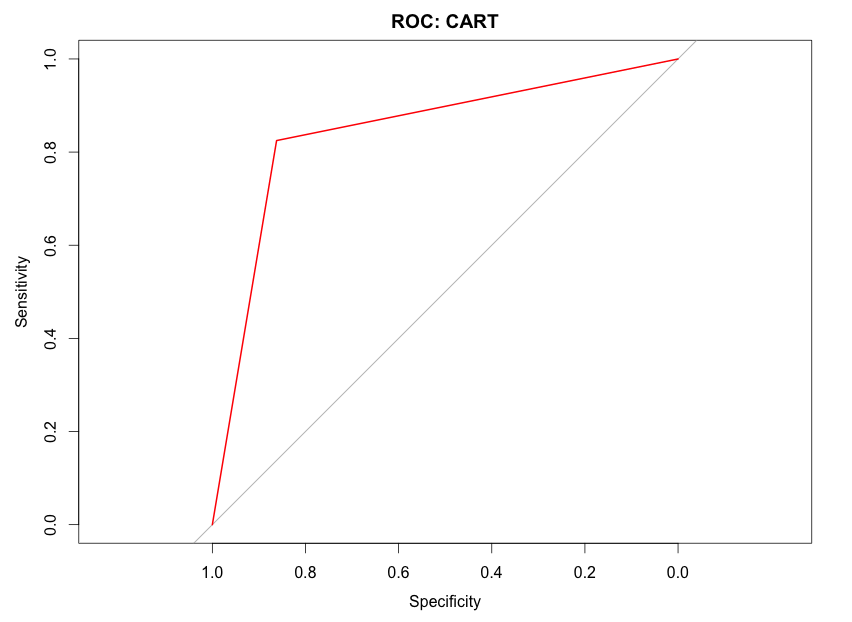
\includegraphics[scale=0.5]{CART_ROC.png}  

%---------------- (SVM)--------------------%
\subsection{SVM}
\begin{Schunk}
\begin{Sinput}
#very slow with R for 100K large data
set.seed(1)
library(e1071)
testing$IsAlert[testing$IsAlert==1] <- "TRUE"
testing$IsAlert[testing$IsAlert==0] <- "FALSE"

svm.fit <- svm(testing[,-c(1,9,27,29)], testing[,1], type="one-classification", kernel="linear", scale=TRUE, nu=0.5)
svm.pred <- predict(svm.fit, testing[,-c(1,9,27,29)])

svm.table <- table(svm.pred, testing$IsAlert)
1-sum(diag(svm.table))/sum(svm.table)

library(pROC)
roc.curve <- roc(as.numeric(svm.pred), as.integer(factor(testing$IsAlert))-1)
plot(roc.curve, main = "Logistic Regression ROC Curve", col = "red")
auc.score<-auc(as.integer(factor(testing$IsAlert))-1, as.numeric(svm.pred))
auc.score
\end{Sinput}
\begin{Soutput}
[1] 0.5706673
\end{Soutput}
\end{Schunk}

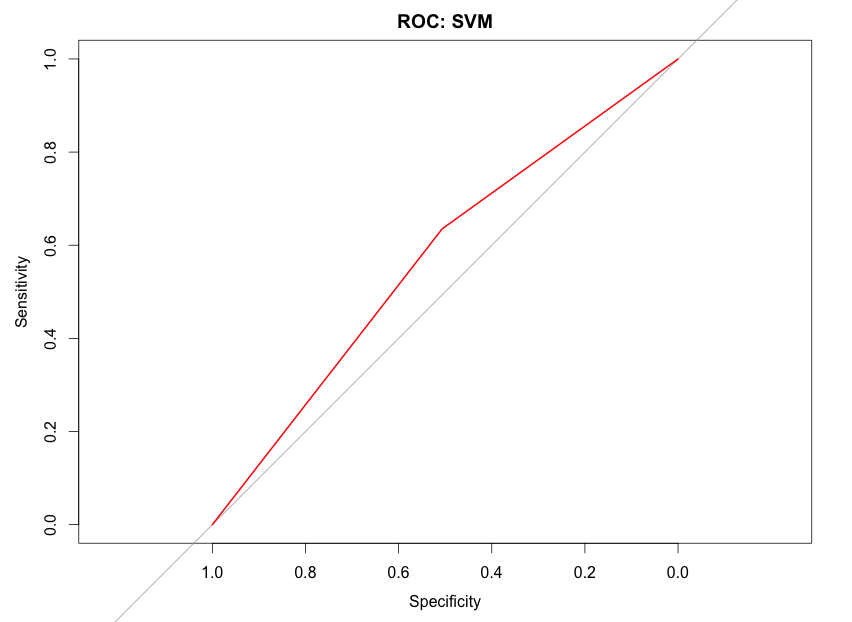
\includegraphics[scale=0.5]{SVM_ROC.png} 

%------------------------------------ (Result) ------------------------------------%
\section{Result}
\begin{table}[ht]
\begin{center}
\begin{tabular}{|l|l|l|l|}
\hline
\textbf{Method} & \textbf{AUC Score} & \textbf{Variables Selected}  & \textbf{Computation Time (s)} \\ \hline
Logistic &  0.78 & 23 vars  & 10.722 \\  \hline
\rowcolor{yellow}
Random Forest &0.93 & V11 E10 E7 & 393.314 \\ \hline
Decistion Tree & 0.83 & V11 E10 P5 P6 V1 &  10.722 \\ \hline
Naive Bayes & 0.76 & -- & --\\ \hline
NN(two layer) & 0.77 & -- & -- \\ \hline
SVM & 0.73 & -- & --\\ 
\hline
\end{tabular}
\end{center}
\end{table}

%------------------------------------ (Summary and Discussion) ------------------------------------%
\section{Summary and Discussion}
We have shown that ensemble method random forest leads to good accuracy in the prediction of when a driver is not alert. Futhermore, only a few features (variables selected) need to be measured to achieve the accuracy.

%------------ References ------------%
\section {References}
[1]  "An Introduction to Statistical Learning" by James, G., Witten, D., Hastie, T., Tibshirani, R. \newline
[2] \url{https://www.kaggle.com/c/stayalert}. \newline
[3] \url{https://www.kaggle.com/c/stayalert/data}. \newline
[4] "First place in the 'Stay Alert!' competiion", inference, March \textit{2011}. \newline
[5] "Stay Alert! The Ford Challenge", L. Fourrier, F. Gaie, T. Rolf. \newline
[6] "Stay Alert! The Ford Challenge", T. Tariq, A. Chen, Fall \textit{2012}. \newline
[7] \url{http://stats.stackexchange.com/questions/76365/examples-for-one-class-svm-in-r}. \newline
[8] \url{https://www.kaggle.com/c/stayalert/forums}. \newline
[9] \url{http://en.wikibooks.org/wiki/LaTeX/Tables}. \newline

%------------ End... ----------------%
%\end{singlespacing}
\end{document}
